
\documentclass[svgnames]{beamer}


\mode<presentation>
{
  \usetheme[titleformat=smallcaps,numbering=fraction,progressbar=frametitle]{metropolis}
  \usecolortheme[light,accent=orange]{solarized}
  %\usecolortheme[named=Goldenrod]{structure}
  % or ...

  \setbeamercovered{transparent}
  % or whatever (possibly just delete it)
}


% \usepackage{mathtext}
\usepackage[utf8]{inputenc}
\usepackage[english,russian]{babel}
\usepackage{cmap}
\hypersetup{unicode=true}
\graphicspath{{images/}{slides/images}}


\title[CMTA 03] % (optional, use only with long paper titles)
{Контрастивный анализ}

\subtitle
{Квантитативный анализ текста} % (optional)

\author%[Author, Another] % (optional, use only with lots of authors)
{Кирилл Александрович Маслинский}
% - Use the \inst{?} command only if the authors have different
%   affiliation.

\institute%[Universities of Somewhere and Elsewhere] % (optional, but mostly needed)
{ЕУ СПб}
% - Use the \inst command only if there are several affiliations.
% - Keep it simple, no one is interested in your street address.

\date%[Short Occasion] % (optional)
{21.02.2022 / 03}

\subject{natural language processing, text mining}
% This is only inserted into the PDF information catalog. Can be left
% out. 


\AtBeginSubsection[]
{
  \begin{frame}<beamer>[plain]{План}
    \tableofcontents[sectionstyle=show/hide,subsectionstyle=show/shaded/hide]
  \end{frame}
}

\newcommand{\tb}[1]{\colorbox{yellow}{#1}\space}
\newcommand{\Sp}[1]{\colorbox{green}{#1}\space}
\newcommand{\Sn}[1]{\colorbox{red}{#1}\space}


\begin{document}

\begin{frame}
  \titlepage
\end{frame}

\section{Ключевые слова}

\subsection{Использование контрастного корпуса}

\begin{frame}
  \frametitle{Метод контрастного корпуса}
  Задача — извлечение лексики, характерной для данного корпуса
  \begin{itemize}
  \item Контрастный корпус (reference corpus) — отражает
    словоупотребление в языке вообще или в более широкой предметной
    области
  \item Составить частотные списки слов для изучаемого и контрастного
    корпуса
  \item Отсортировать слова по расхождению частотности с ожидаемой
    на основании контрастного корпуса
  \item Ключевые слова изучаемого корпуса — наверху списка
  \end{itemize}
\end{frame}


\begin{frame}
  \frametitle{Ключевые слова корпуса}
  \begin{block}{Simple maths (by Adam Kilgarriff)}
  «это слово встречается в этом корпусе вдвое чаще, чем в том»
\end{block}
\begin{itemize}
\item Самый простой подход
  \begin{itemize}
  \item Нормализовать частотности
    \begin{itemize}
    \item употреблений на тысячу или употреблений на миллион (IPM)
    \end{itemize}
  \item Вычислить отношение нормализованных частотностей
  \item Отсортировать список слов по значению отношения
  \end{itemize}
\end{itemize}
\end{frame}

\begin{frame}
  Для примера: 
\begin{itemize}
\item Два корпуса по миллиону токенов
\item Нормализовать частотности не нужно
\item[\textbf{fc}] focus corpus — изучаемый корпус
\item[\textbf{rc}] reference corpus — контрастный корпус
\end{itemize}
\end{frame}

\begin{frame}
  \frametitle{Проблема 1:  нельзя делить на 0}
  \begin{tabular}[l]{lccc}
    слово & fc & rc & отношение \\
    \hline
    редкость & 10 & 0 &  ? \\
    помешивать & 100 & 0 &  ? \\
    вкуснотища & 1000 & 0 &  ? \\
  \end{tabular}

Стандартное решение: прибавить 1:

  \begin{tabular}[l]{lccc}
    слово & fc & rc & отношение \\
    \hline
    редкость & 11 & 1 &  11 \\
    помешивать & 101 & 1 &  101 \\
    вкуснотища & 1001 & 1 &  1001 \\
  \end{tabular}
\end{frame}

\begin{frame}
  \frametitle{Проблема 2: из-за редких слов слишком много больших
    отношений}
  Частотность тоже важна.   Решение: прибавить n.

  \begin{itemize}
  \item $n=1$

  \begin{tabular}[l]{lcccccc}
    слово & fc & rc & fc+n & rc+n & отношение & ранг \\
    \hline
    изредка & 10 & 0 & 11 & 1 & 11,00 & 1 \\
    временами & 200 & 100 & 201 & 101 & 1,99 & 2 \\
    часто & 12000 & 10000 & 12001 & 10001 & 1,20 & 3 \\
  \end{tabular}
  
  \item $n=100$

  \begin{tabular}[l]{lcccccc}
    слово & fc & rc & fc+n & rc+n & отношение & ранг \\
    \hline
    временами & 200 & 100 & 300 & 200 & 1,50 & 1 \\
    изредка & 10 & 0 & 110 & 100 & 1,10 &  3 \\
    часто & 12000 & 10000 & 12100 & 10100 & 1,20 & 2 \\
  \end{tabular}

  \end{itemize}
  
\end{frame}

\subsection{Отношение правдоподобия}

\begin{frame}
  \frametitle{Уходящая эпоха статистической значимости}
  \centering
  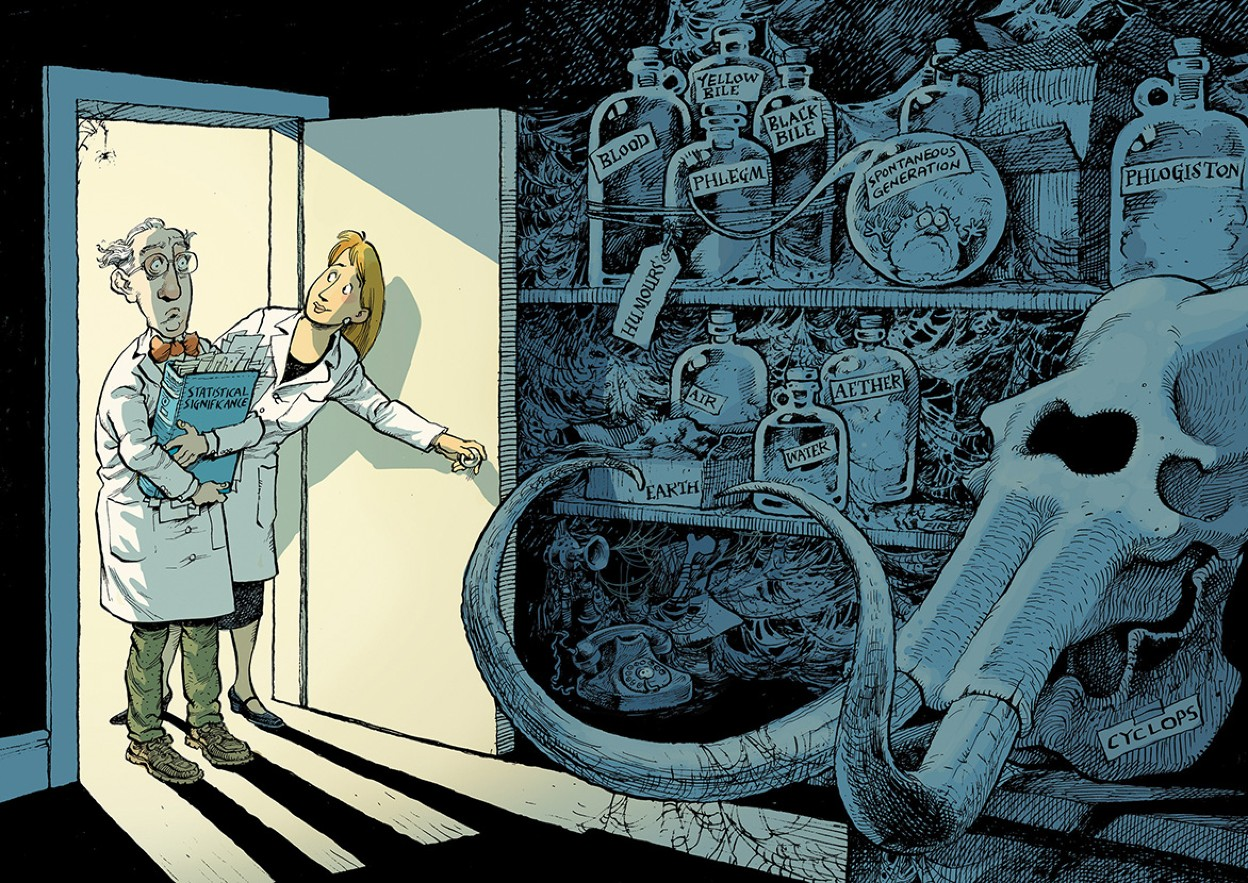
\includegraphics[width=.9\textwidth]{significance}
  \footnotesize
  \href{https://www.nature.com/articles/d41586-019-00857-9}{Amrhein et
    al. “Scientists rise up against statistical significance” 
    (2019)}
\end{frame}

\begin{frame}
  \frametitle{Нормальность и распределение слов}
  В парадигме стандартных статистических тестов при сравнении
  частотностей слов возникали проблемы:
  \begin{itemize}
  \item Предположение о нормальности неверно в случае частотного
    распределения слов
  \item В языке слишком много редких событий
  \item Неприменимость тестов, основанных на предположении о
    нормальности (напр., хи-кавдрат), как минимум к редким событиям (частотность < 5)
  \end{itemize}
\end{frame}

\begin{frame}
  \frametitle{Нормальное распределение излишне удивлено}
  \centering
  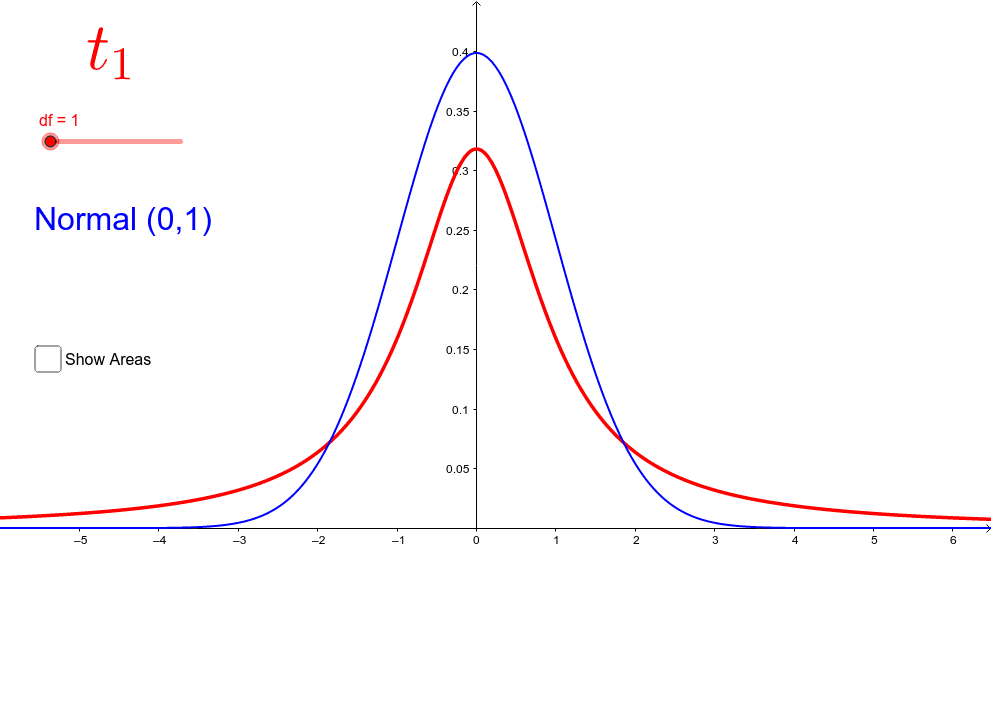
\includegraphics[width=\textwidth]{normal-student}
\end{frame}

\begin{frame}
  \frametitle{Отношение правдоподобия: мотивировка}
  \framesubtitle{Log likelihood ratio}
  Способ включить частотности слов в парадигму статистических тестов:

  \href{https://aclanthology.org/J93-1003.pdf}{Ted Dunning “Accurate
    Methods for the Statistics of Surprise and Coincidence” (1994)}
  \begin{itemize}
  \item Отношение правдоподобия менее зависит от предположения о
    нормальности распределения данных
  \item Поэтому не так резко завышает значимость редких событий и
    может применяться для оценки различий не только самых частотных слов
  \end{itemize}
\end{frame}

\begin{frame}
  \frametitle{Отношение правдоподобия: формула}
  \begin{tabular}[c]{|p{.3\textwidth}|c|c|c|}
    \hline
   & Корпус 1 & Корпус 2 & Всего \\
    \hline
    Частотность слова & a & b & a+b \\
    \hline
    Частотность остальных слов & c-a & d-b & c+d-a-b \\
    \hline
    Всего & c & d & c+d \\
    \hline
  \end{tabular}

\bigskip
  Ожидаемые частотности:
  \begin{itemize}
  \item[E1] $\frac{c}{c+d}(a+b)$
  \item[E2] $\frac{d}{c+d}(a+b)$
  \end{itemize}

  \begin{equation}
    LL = G^2 = 2 (a \log (a/E1) + b \log (b/E2) ) 
  \end{equation}
\end{frame}

\begin{frame}
  \frametitle{Проблема Log-Likelihood}
  \begin{itemize}
  \item Более чувствителен к частотным событиям (словам), чем к менее
    частотным [занижает степень различия по менее частотным словам]
  \end{itemize}
\end{frame}

\begin{frame}[standout]
  \alert{Эксперимент на царях и цветочках}
\end{frame}

\begin{frame}[standout]
  \frametitle{Практический вывод}
  
\includegraphics[height=.8\textheight]{statistics_2x.png}
\end{frame}

\subsection{Логарифм отношения шансов}

\begin{frame}
  \frametitle{Шансы (odds)  вероятность}
  \Large
  \centering
  \begin{description}
  \item[шансы] \textcolor{red}{1} : \textcolor{blue}{3} 
  \item[вероятность] \textcolor{red}{1/4} , \textcolor{blue}{3/4}
  \item[шансы красных] \textcolor{red}{1} : 3 = 0,33
  \item[вероятность красных] \textcolor{red}{1}/4 = 0,25
    \pause
  \item[шансы через вероятность] $p/(1-p) = 0,25 / (1 - 0,25) =
    \textcolor{red}{1}/4 : \textcolor{blue}{3}/4 = 0,33$
  \end{description}  
\end{frame}

\begin{frame}
  \frametitle{Два события: отношение шансов}
  \Large
  \begin{description}
  \item[шансы1] \textcolor{red}{1} : 3 = 0,33
  \item[шансы2] \textcolor{red}{2} : 5 = 0,4
  \item[шансы1/шансы2] 1/3 : 2/5 = 5/6 = 0,83
  \item[шансы2/шансы1] 2/5 : 1/3 = 6/5 = 1,2
  \end{description}
\end{frame}

\begin{frame}
  \frametitle{Логарифм отношения шансов}
  \Large
  \begin{description}
  \item[шансы1/шансы2] $\log (5/6) = -0,18$
  \item[шансы2/шансы1] $\log (6/5) = 0,18$
  \end{description}
\end{frame}

\begin{frame}
  \frametitle{Шансы на логарифмической шкале}
  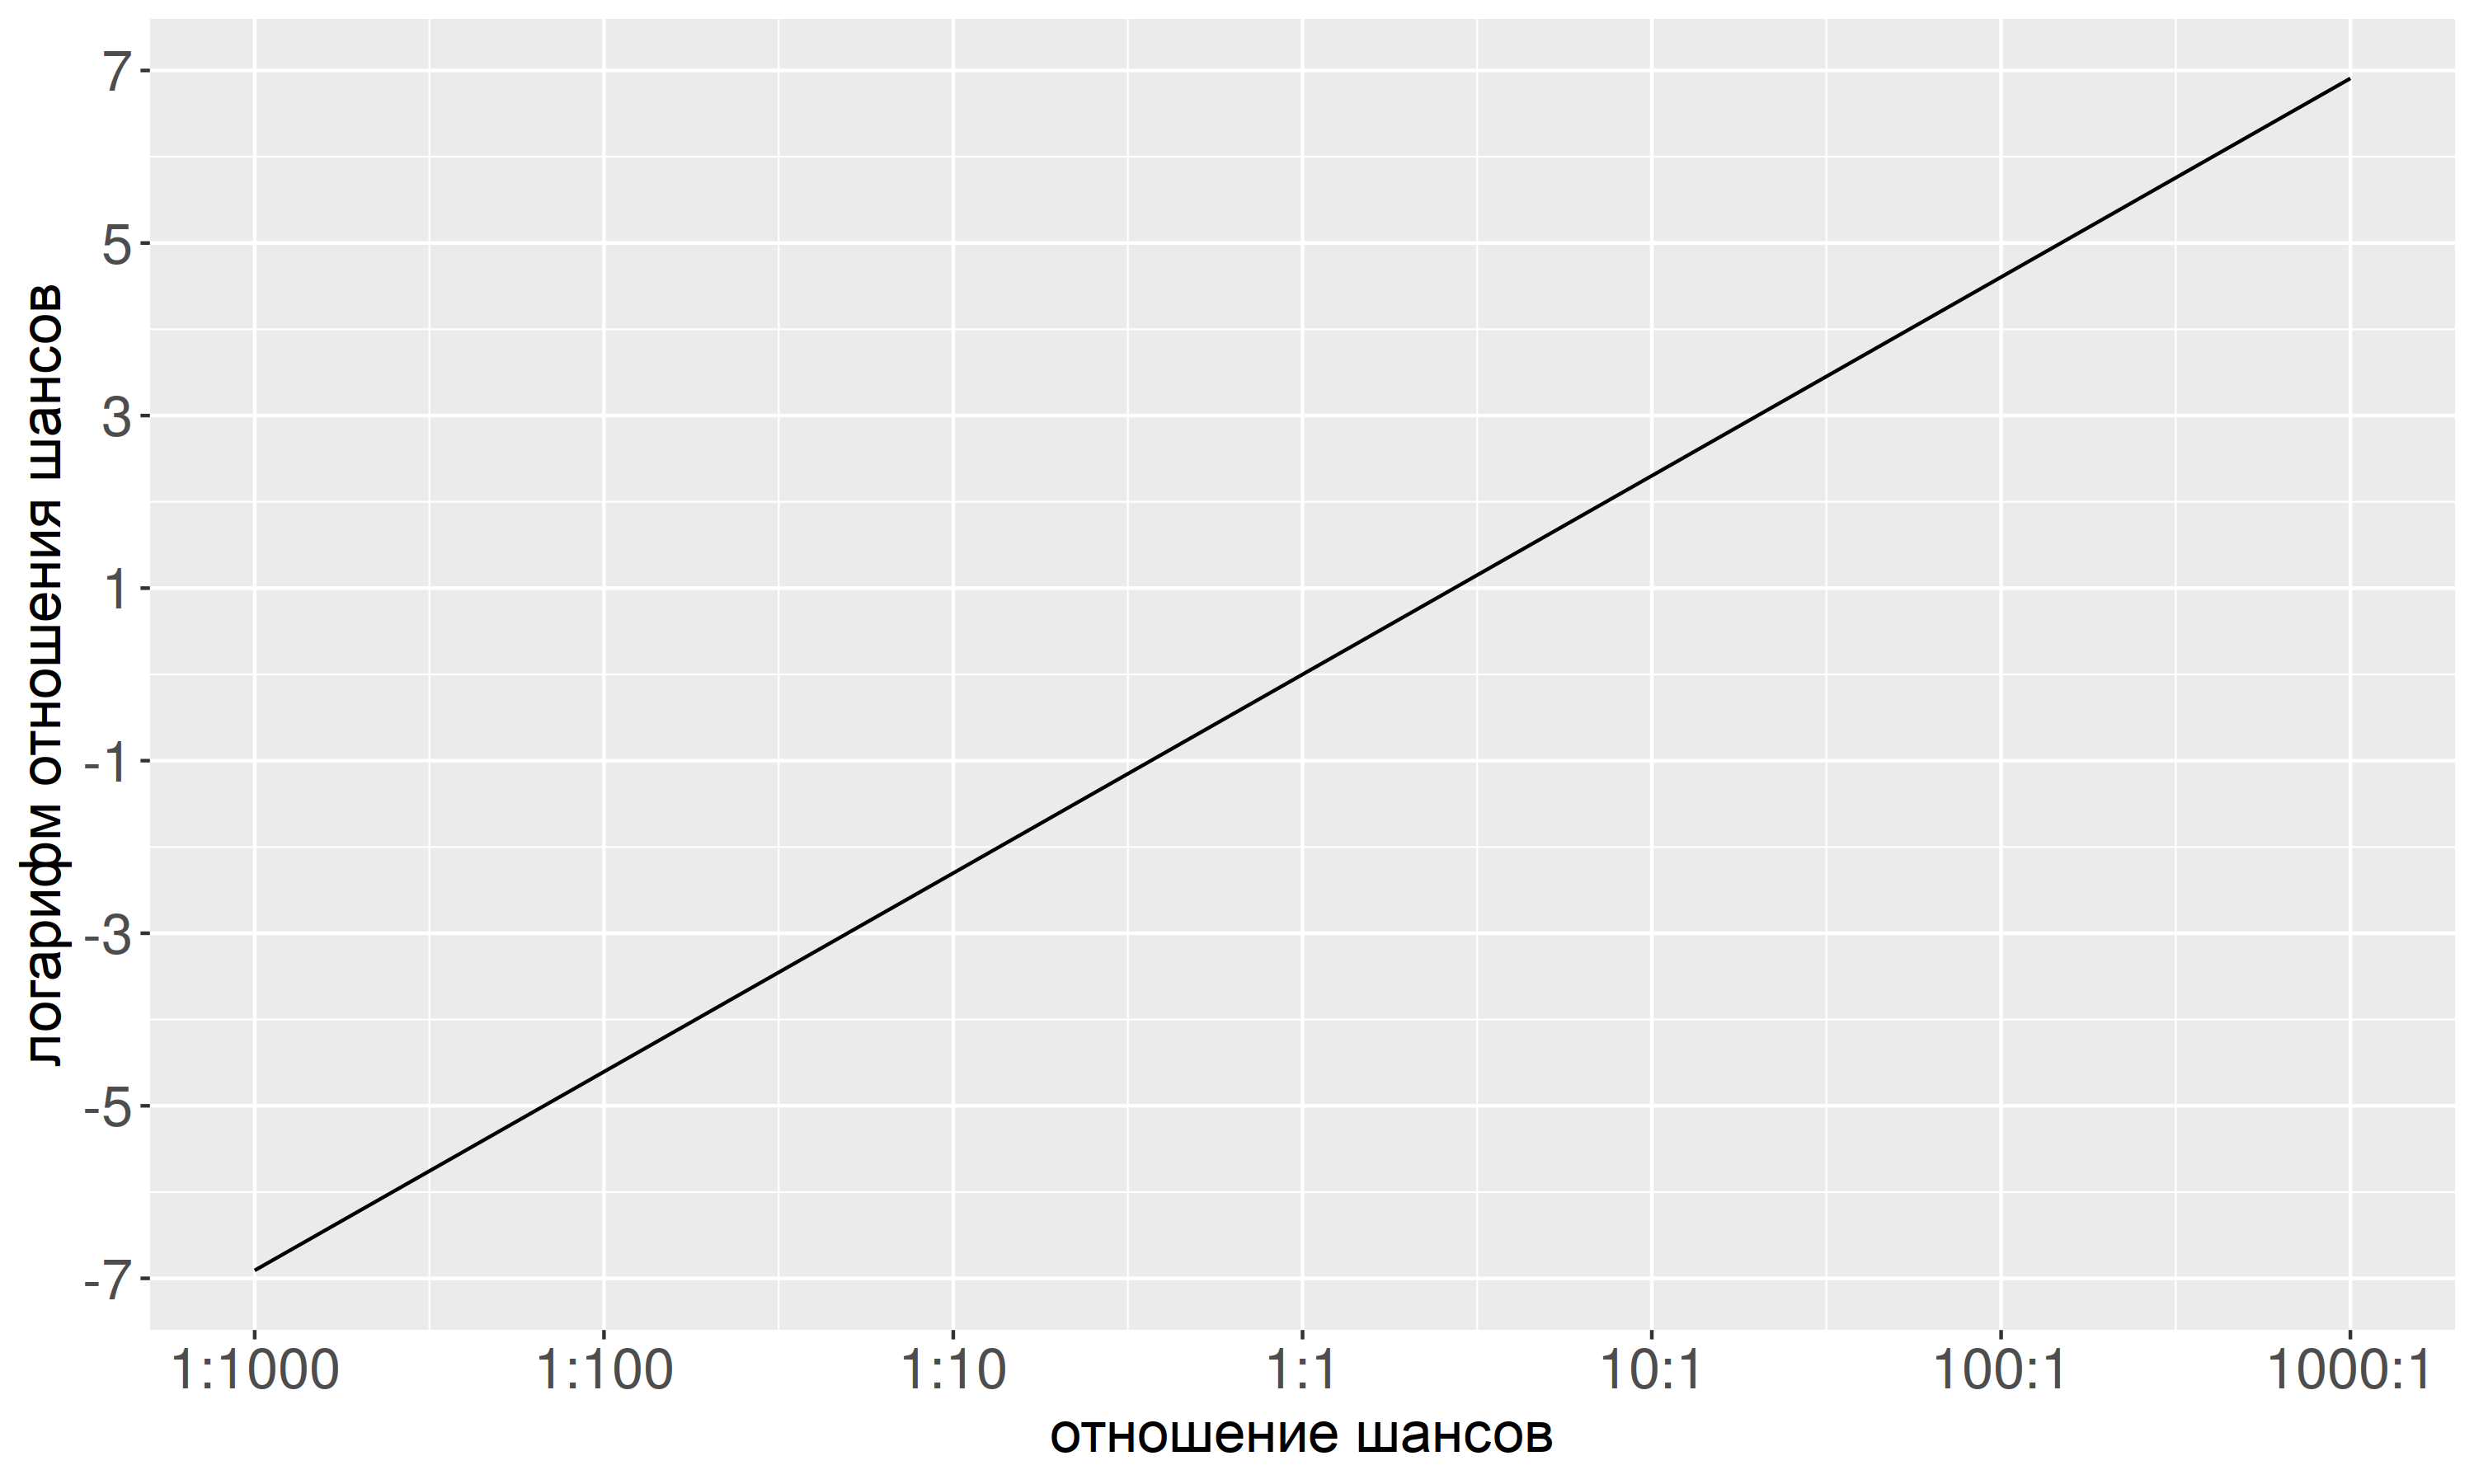
\includegraphics[width=\textwidth]{logodds}
\end{frame}

\subsection{Взвешенное отношение шансов}


\begin{frame}
  \frametitle{tidylo by Julia Silge: weighted log odds}
  \LARGE
  % Weighted by uninformative Dirichlet prior:
    $$
    \delta =
    \frac{\frac{f_{(w,c1)}+\textcolor{red}{\alpha_{(w,c1)}}}{N_{c1}+\textcolor{red}{\alpha_{c1}}-f_{(w,c1)}-\textcolor{red}{\alpha_{(w,c1)}}}}{\frac{f_{(w,c2)}+\textcolor{red}{\alpha_{(w,c2)}}}{N_{c2}+\textcolor{red}{\alpha_{c2}}-f_{(w,c2)}-\textcolor{red}{\alpha_{(w,c2)}}}}
    $$
\end{frame}


\end{document}
